\documentclass[11pt]{article} % use larger type; default would be 10pt

\usepackage[utf8]{inputenc} % set input encoding (not needed with XeLaTeX)


\usepackage{geometry} % to change the page dimensions
\geometry{a4paper} % or letterpaper (US) or a5paper or....

\usepackage{graphicx} % support the \includegraphics command and options
\usepackage{amsmath}


\usepackage{booktabs} % for much better looking tables
\usepackage{array} % for better arrays (eg matrices) in maths
\usepackage{paralist} % very flexible & customisable lists (eg. enumerate/itemize, etc.)
\usepackage{verbatim} % adds environment for commenting out blocks of text & for better verbatim
\usepackage{subfig} % make it possible to include more than one captioned figure/table in a single float

\usepackage{fancyhdr} % This should be set AFTER setting up the page geometry
\pagestyle{fancy} % options: empty , plain , fancy
\renewcommand{\headrulewidth}{0pt} % customise the layout...
\lhead{}\chead{}\rhead{}
\lfoot{}\cfoot{\thepage}\rfoot{}

\usepackage{sectsty}
\allsectionsfont{\sffamily\mdseries\upshape} % (See the fntguide.pdf for font help)

\usepackage[nottoc,notlof,notlot]{tocbibind} % Put the bibliography in the ToC
\usepackage[titles,subfigure]{tocloft} % Alter the style of the Table of Contents
\renewcommand{\cftsecfont}{\rmfamily\mdseries\upshape}
\renewcommand{\cftsecpagefont}{\rmfamily\mdseries\upshape} % No bold!
\newcommand{\strong}[1]{\textbf{#1}}
\newcommand{\code}[1]{\texttt{#1}}
\newcommand{\st}{$^{\text{st}\ }$}
\newcommand{\nd}{$^{\text{nd}\ }$}
\newcommand{\rd}{$^{\text{rd}\ }$}
\newcommand{\nth}{$^{\text{th}\ }$}

\title{Assignment 4}
\author{Nathan Jervis}

\begin{document}
\maketitle

\section{Question 4.4}

\subsection{Part A}

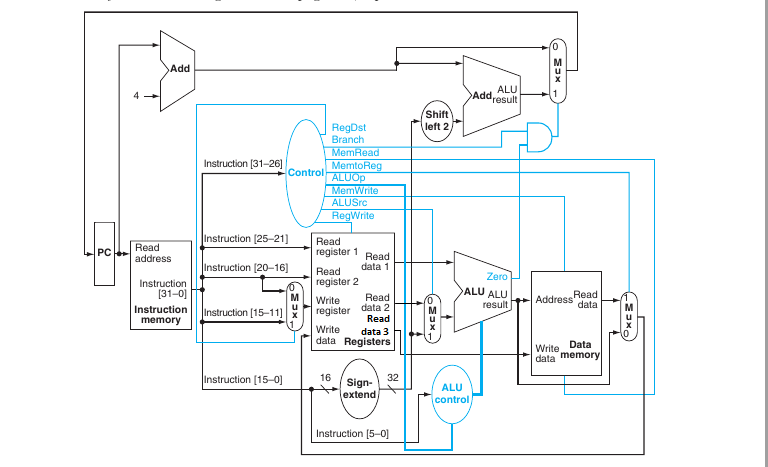
\includegraphics[width=\textwidth]{CPU3.png}

We can re-use the write register selection as the selection for a 3\rd read register. This read register is used as the write data now, instead of the 2\nd one like the previous diagram. We can make this transistion since the only opcode which currently uses that data line is \code{sw}. All we need to do is ensure that for \code{sw} the \strong{RegDst} control pin is set to 0, so the [20-16] part of the opcode is used as the write register selection. Since we've already repurposed this to read into the new 3\rd register line, it will still output the same information to the \emph{write data} section of the memory unit. \code{swr} will have \strong{RegDst} set to 1, and will therefore use the [15-11] part of the opcode to select which register to write.

Adding this new command \code{swr} requires reading from a 3\rd register, but it does not need any additional control lines, and doesn't even add new wiring to the circuit (besides what's required inside the register file to read from a 3\rd register that is). 

\subsection{Part B}

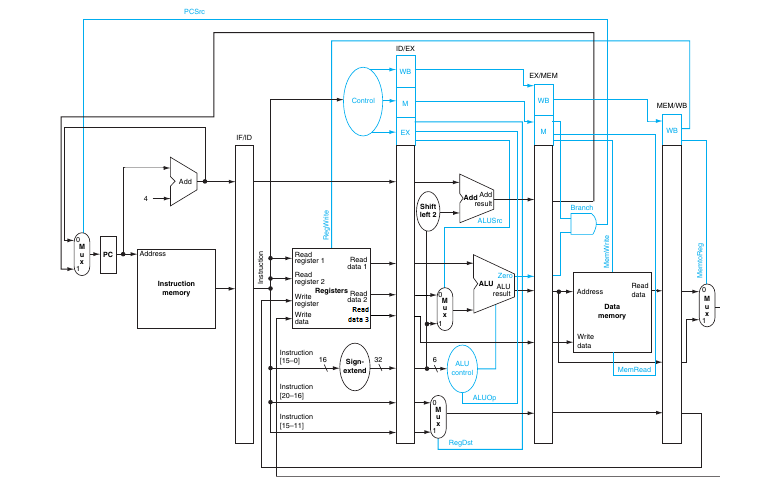
\includegraphics[width=\textwidth]{pipelineCPU2.png}

This picture is very similar to the previous one. Again the only change required is to use the write register selector to select a 3\rd  register to read from. The pipelined version also additionally requires a new spot to hold the register data between the \emph{Instruction Decode} and the \emph{Execute} stages (the one to hold the data between \emph{Execute} and \emph{Memory} already was there).

\subsection{Part C}

There are no new hazards introduced, just slightly different things to look out for. \code{lwr} has basically the same hazards as any arithmetic operation such as \code{add} (it may make a difference for optimization sake that \code{lwr} loads from memory, ie to prefetch it, but it doesn't introduce new hazards). \code{swr} is a little bit of an oddball since it now reads from a 3\rd register, and this will have to be kept in mind, but it doesn't introduce any new types of hazards, just a 3\rd spot to check for read hazards in this instruction (whereas normally it'd only check the 3\rd register for write hazards).


\section{Question 4.5}

\emph{Note: I'm assuming for these questions we're using the original CPU as in the textbook, and not the new one with \code{swr} and \code{lwr}}

\subsection{Part A}

Cross talk between \emph{RegDst} and \emph{MemWrite}, causing them to be the logical \strong{AND} of the 2 inputs. The only case when \emph{MemWrite} is 1 is when the \code{sw} opcode is used. In this case \emph{RegDst} is 0, which means with this cross-talk both \emph{RegDst} and \emph{MemWrite} will always be \code{0/false} which will cause disastrous consequences for code (as \code{sw} will never actually write it's data, and all registers which are supposed to use the 3\rd register to write to end up using the 2\nd instead, which is all \emph{r-format} instructions. In order to detect this problem the following code can be used:

\begin{verbatim}
	ori $t0 $zero 1
	ori $t1 $zero 2
	add $
\end{verbatim}
\end{document}
